\documentclass[12pt,letterpaper]{article}

\title{Puget Sound CS Mentoring Event Poster 2}

\usepackage{hyperref}
\usepackage{setspace}
\usepackage{amsmath}%
\usepackage{MnSymbol}%
\usepackage{wasysym}%
\usepackage{lmodern}


\usepackage[utf8]{inputenc}
\usepackage[T1]{fontenc}
\usepackage[sfdefault,lf]{carlito}

\usepackage[margin=1.1cm,letterpaper]{geometry}
\usepackage{multicol}
\usepackage{ragged2e}
\usepackage{tabularx}
\usepackage[table]{xcolor}
\usepackage{graphicx}

%cyan 36a8b8
%blue b2d4ef
%purple c677dd
%overleaf green 4F9C45
%green 7b9e62
%red 1 cb4752
%red 2 be5046
%orange 1 d19a66
%orange 2 e5c07b

\definecolor{HighlightColor}{HTML}{d19a66}
\graphicspath{{img/}}
\pagestyle{empty}
\RaggedRight
\parskip=12pt plus 4pt

\begin{document}


{\fontsize{40pt}{42pt}\bfseries\selectfont\color{HighlightColor}%
Build A Professional Showcase
\\}% 
%\begin{flushright}
~\hfill
{\LARGE\bfseries%
\mbox{2pm Sunday April 30, 2017 @ the math lounge}%
}
%\end{flushright}


%

{\centering%
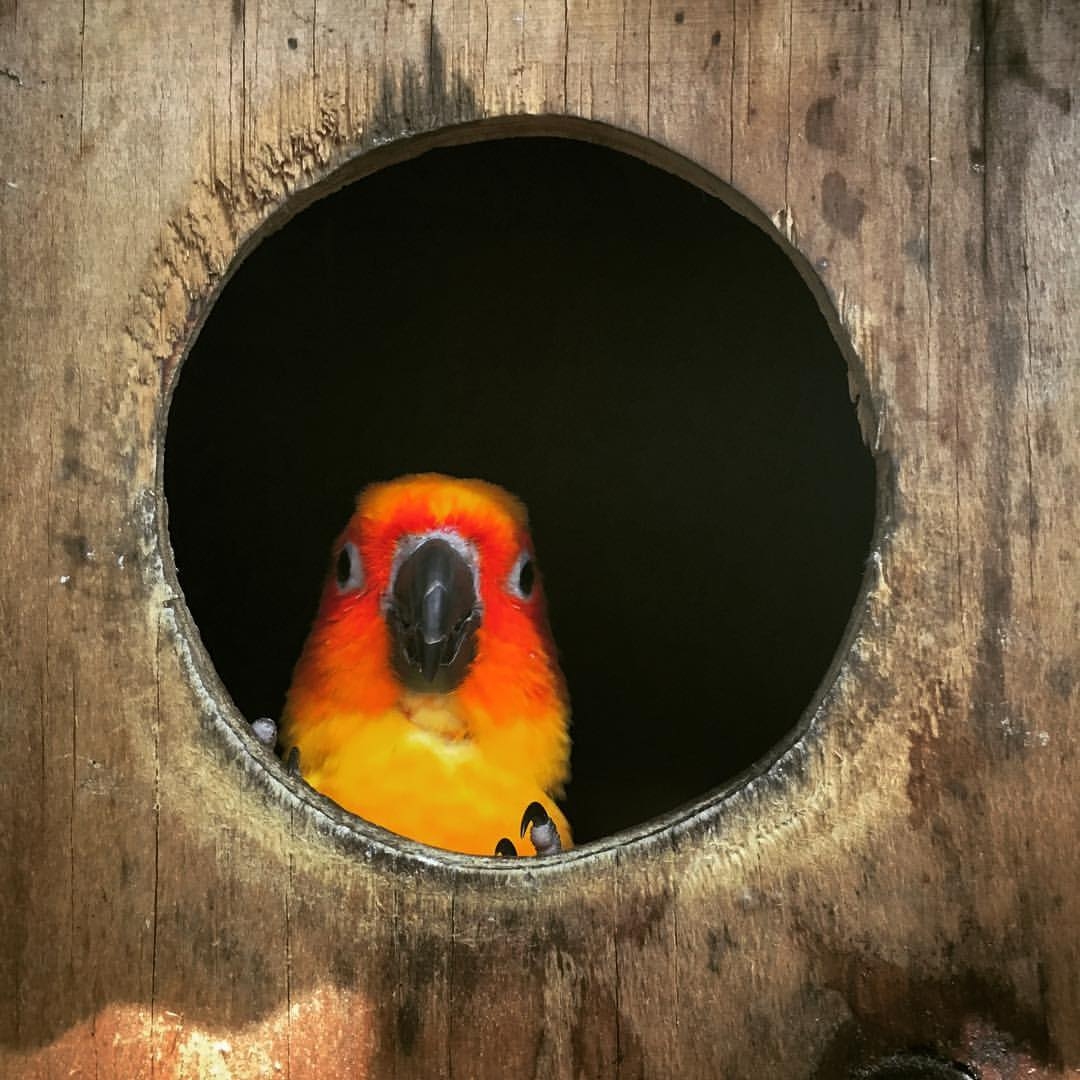
\includegraphics[width=0.93\linewidth,trim={3cm 5cm 5cm 3cm}, clip]{hello_bird}%
\par}


%{\hfill\LARGE\bfseries Come get social!}\par%
%\vfill
\vspace{-3ex}
\begin{large}
\justify
{\setstretch{0.9} Come join us for an hour-long resume-crafting and \texttt{github.io} boot camp. A few (really rad) upperclassmen will lead a hands-on tutorial on showcasing your talents in a resume and making yourself a \texttt{github.io} page to display it on. We'll walk you through step-by-step and help you make your professional web presence your own. Plus, we'll have snacks! Whether you are totally new to programming or have been around the block a few times, we want to see you there! We are looking forward to building social connections between new members of the CS department and older students.\par}

\end{large}


%\vfill

{\LARGE Questions?}
\hfill
{\Large Contact Matthew Moreno \url{mamoreno@pugetsound.edu}}
\end{document}